% \documentclass{beamer}
\documentclass[pdf,10pt]{beamer}
% \usetheme{Copenhagen}
% \usetheme{metropolis}           % Use metropolis theme
\usetheme[progressbar=foot,numbering=counter,titleformat=smallcaps,sectionpage=none]{metropolis}
\usepackage{graphicx}
\usepackage{url}
\usepackage{amsmath}
\usepackage{subeqnarray}
\usepackage{empheq}
\usepackage{color}
\usepackage{mathtools}

% \usepackage{algorithm}
% \usepackage{algpseudocode}
\usepackage{caption}
% \usepackage{subcaption}
\usepackage{multirow}

\usepackage{amssymb}
\usepackage{subfigure}

\usepackage{tikz}
\usetikzlibrary{arrows.meta,shapes.arrows}

% \usepackage{todonotes}
% \newcommand{\textcomment}[1]{\todo[inline]{#1}}
% \newcommand{\footcomment}[1]{\footnote{\todo[inline]{#1}}}

\usepackage{biblatex}
\bibliography{beijing}

% filled boxes like theorem etc
\metroset{block=fill}


\begin{document}

% \title{Verifying properties on a discrete topological city space}
\title{\fontsize{14pt}{10}\selectfont Spatial model checking with microservices for the internet-of-things}

% \author{\textbf{Carlo Ghezzi and Christos Tsigkanos } }
\institute{\fontsize{9pt}{10}\selectfont Politecnico di Milano, Italy} 
% \date{\today}
% \logo{\includegraphics[width=0.25\textwidth]{img/polimi.png}}

\begin{frame}
\titlepage
\end{frame}








\begin{frame}[t]\frametitle{Setting}
\centering
% \vspace{3.5cm}

\begin{itemize} 

\item Wide deployments of internet-enabled things within smart applications (i.e. smart cities)
\item Complex relations between locations of things with respect to their environment may arise
\item Things change location; location may affect satisfaction of system requirements
 \end{itemize}
\pause
% , location and relation between
% \fontsize{9cmpt}{10}\selectfont
\textbf{How can we \textcolor{mLightBrown}{enable runtime verification} of requirements of space-dependent systems of internet-of-things? }
\pause
\vspace{0.2cm}
\begin{itemize} 
\fontsize{9pt}{10}\selectfont
 \item Properties expressing arbitrary relations in space are known upfront
 \item We seek formal assurances that properties hold in a given space-things configuration 
 \end{itemize}

 Verify spatial properties on configurations of city space populated with locations of things at given point
\end{frame}

















\begin{frame}[t]\frametitle{Topological abstraction}
\vspace{2.6cm}
\textcolor{mLightBrown}{Key intuition:} Space is composed of relations between entities
\begin{itemize} 
 % \item Computational topology represents the 
 \item Evaluation model is a discrete graph structure \\representing a topological view of space 
 \item Serves as the critical abstraction step 
\item Enables formal specification and verification techniques
 \end{itemize}
\end{frame}









% \begin{frame}[t]\frametitle{Analysis: Spatial Model Checking}
\begin{frame}[t]\frametitle{Expressing \& Verifying Properties}

A \textcolor{mLightBrown}{spatial logic} can express complex properties of space and enable automated verification. For example: %and an automated 

\begin{exampleblock}{Example}
From the location where a taxi is near a gas station, is there a way to go to a metro station going through --an arbitrary number of-- bus stops? 
\end{exampleblock}


\begin{exampleblock}{Example}
From which locations where taxis are near a pharmacy, we can reach a bar through metro stations and bus stops, without going near a hospital? 
\end{exampleblock}

\textbf{We can support logic-based reasoning }
\begin{itemize}
\item Formal specification of properties
 \item Spatial properties may be non trivial
\end{itemize}
\end{frame}







\begin{frame}[t]\frametitle{Spatial Evaluation Model}
\begin{enumerate}
 \item Generate a \textcolor{mLightBrown}{closure space} from the accessibility graph
 \item Equip with a \textcolor{mLightBrown}{valuation function} associating points with atomic propositions (POIs, taxis etc)
 \item Big-step semantics: \textcolor{mLightBrown}{truth values of spatial relations} or \textcolor{mLightBrown}{points where spatial relations hold} % in model
\end{enumerate}
Spatial Logic for Closure Spaces\footfullcite{ciancia2014specifying}
\begin{subequations}
\begin{empheq}[]{align}   
\tau ::= \mathsf{p} ~|~ \top ~|~ \neg \tau ~|~  \tau \wedge  \tau ~|~ \mathcal{C}\ \tau ~|~  \tau\ S\  \tau \nonumber
\end{empheq} 
\end{subequations}
\vspace{-0.5cm}
% \end{small}    
\begin{itemize}
\item Closure \textcolor{mLightBrown}{"one step"} modality
\item \textcolor{mLightBrown}{Surrounds} modality %(spatial interpretation of "until")% on closure space points
 % \item Propositions $p$ are parametric \textcolor{mLightBrown}{bigraphical patterns}
\end{itemize}

\end{frame}






\begin{frame}[t]\frametitle{Modelling complex properties in space\footfullcite{fse17}: reachability}
\begin{footnotesize}




 % {\em Weak reachability}: 
 Notion of path in a closure space
   \begin{empheq}[]{align}
    \label{weakreach}
      & \phi\ \mathcal{R}\ \psi \overset{def}= \neg \big((\neg\psi)\ \mathcal{S}\ (\neg\phi)\big) \nonumber
    \end{empheq} 

% Example: $\mathsf{Spool}$ is reachable from a 
% $\mathsf{Room}$ in which a $\mathsf{Printer}$ is located
%       \begin{empheq}[]{align}
%     \label{reach-example}
%       \mathsf{Room}_?(\mathsf{Printer}_?~|~-_{0}))\ \mathcal{R}\ \mathsf{Spool}_? \nonumber
%     \end{empheq} 

% {\em Strong reachability}: 
Constrain the traversed path
      \begin{empheq}[]{align}
    \label{weakreach}
      & \phi\ \mathcal{T}\ \psi \overset{def}= \phi \wedge \big((\phi \vee \psi )\ \mathcal{R}\ \psi \big)\nonumber
    \end{empheq} 

% {\em Reach through}: 
Predicate on entities encountered on the traversed path  
% \textcomment{CG: 
      \begin{empheq}[]{align}\label{reachthrough}
     & \phi\ \mathcal{\Re}(\psi)\  \zeta \overset{def}=\phi\ \mathcal{T}\ \big( (\psi\ \mathcal{T}\ \zeta) \wedge (\psi\ \mathcal{T}\ \phi)\big) \nonumber
    \end{empheq} 

% {\em Reach through}: 
Nearness as nested applications of closure operator
% \textcomment{CG: 
      \begin{empheq}[]{align}\label{nearness}
     & \mathcal{N}_n \phi \overset{def}= C_{n} C_{n-1}.. \phi \nonumber
    \end{empheq} 
\end{footnotesize}
\end{frame}



\begin{frame}[t]\frametitle{Modelling complex properties in space}
\begin{footnotesize}


\begin{exampleblock}{Example}
From the location where a taxi is near a gas station, is there a way to go to a metro station going through --an arbitrary number of-- bus stops? 
\end{exampleblock}

 \begin{empheq}[]{align}\label{sp2}
     & \mathsf{taxi}\ \mathcal{\Re} \big(transportbusstop\big)\ \mathsf{transportsubway} \wedge \mathcal{N}_n \mathsf{transportfuel}. \nonumber
    \end{empheq} 
\begin{exampleblock}{Example}
From which locations where taxis are near a pharmacy, we can reach a bar through metro stations and bus stops, without going near a hospital? 
\end{exampleblock}

 \begin{empheq}[]{align}\label{sp2}
     & \mathsf{taxi}\ \mathcal{\Re} \big(transportbusstop \vee transportsubway \wedge !(\mathcal{N}_n healthhospital)\big)\ \nonumber\\ 
     & \mathsf{foodbar} \wedge \mathcal{N}_n \mathsf{healthpharmacy}. \nonumber
    \end{empheq} 
\end{footnotesize}

\end{frame}




\begin{frame}[t]\frametitle{Evaluation \& Datasets}
\vspace{2cm}
Intuition:
\begin{itemize} 
 \item Trajectory datasets can provide movement data points
 \item Points-of-interest datasets can provide static graphs
 \end{itemize}
\begin{exampleblock}{Combining both }
\textbf{Movement data points over time, over a closure space}
\end{exampleblock}
\end{frame}









\begin{frame}[t]\frametitle{Jing Yuan et al Dataset}

T-Drive trajectory dataset\footfullcite{yuan2011driving,yuan2010t}
% \footfullcite{yuan2010t}
\begin{itemize} 
 \item trajectories of 10k taxis over one week
 \item 15M data points
 \item 9M kilometers total distance 
 \end{itemize}
 % Notable ``landmarks'' approach~\footfullcite{yuan2011driving}

OpenStreetMap points-of-interest in Beijing
\begin{itemize} 
\item Various landmarks, public services, shops, etc
 \item e.g. 11741 POIs
 \end{itemize}
\end{frame}


\begin{frame}[t]\frametitle{Obtaining a topological model: process}
\vspace{0.45cm}
\begin{center}
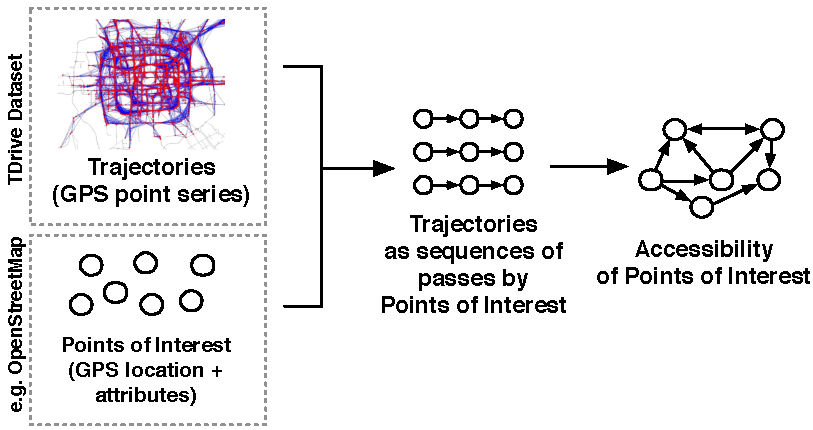
\includegraphics[width=1\textwidth]{img/cl1.pdf}
\end{center}
% \vspace{-0.44cm}
\end{frame}










\begin{frame}[t]\frametitle{Obtaining a topological model: process}
\vspace{-0.35cm}
\begin{center}
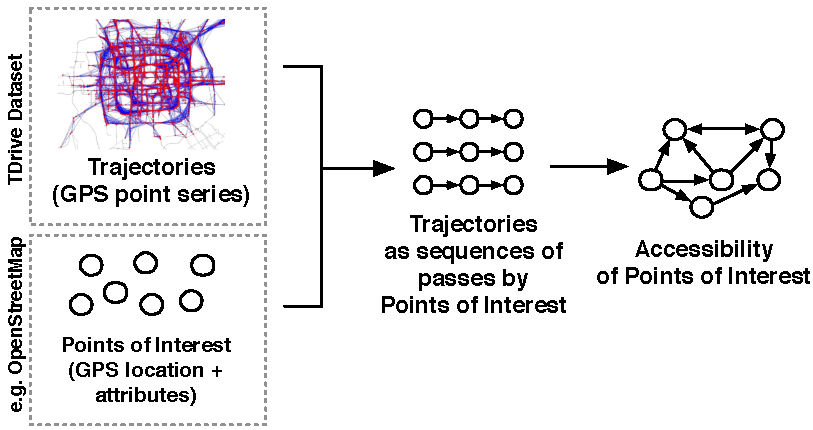
\includegraphics[width=0.75\textwidth]{img/cl1.pdf}
\end{center}
\vspace{-0.44cm}
\begin{enumerate} 
 \item T-Drive trajectory dataset
 \item Points-of-Interest
 \item Discover points that trajectories pass through
 \end{enumerate}
\vspace{-0.24cm}

 \textcolor{mLightBrown}{Key idea:} if an entity's trajectory passes from a point to another, then these points are connected 
\vspace{-0.14cm}
 \begin{itemize} 
 \item We obtain connectivity of points as a graph structure
 \item Nodes are Points-of-Interest %, propositions encode information
 \item Edges reflect ``accessibility'' of a node from another
 \end{itemize}
\end{frame}






\begin{frame}[t]\frametitle{Evaluation Dataset}
\vspace{2cm}
Discrete presences of taxis in Beijing over time
\begin{itemize} 
 \item Taxis move between various points of interest
 \item Can consider them as position \emph{updates} to the global topological space of Beijing
 \end{itemize}
\begin{exampleblock}{Intuition }
\textbf{Every taxi presence triggers a check of a global spatial property} % that the system has to satisfy}
\end{exampleblock}
\end{frame}



\begin{frame}[t]\frametitle{Evaluation Dataset: A property}

``Always from where taxis are near metro stations, there is a way to go to gas stations going through --an arbitrary number of-- bus stops or bars ''
        % '/check/R%28%5Btaxi%5D%2C%28%5BTRANSPORTSUBWAY%5D%20%7C%20%5BTRANSPORTBUSSTOP%5D%29%2C%5BFOODBAR%5D%29%20%26%20%28N%20%5BTRANSPORTFUEL%5D%29%20')


% a: (\mathsf{taxi} \wedge \mathcal{N}_n \mathsf{transportsubway})

% b: (\mathsf{transportbusstop} \vee \mathsf{foodbar})

% e: (\mathsf{transportfuel})
% Let R(a,b,e) = 

\begin{exampleblock}{Formulation}
$(\mathsf{taxi} \wedge \mathcal{C} \mathsf{transportsubway}) \wedge \neg((\neg( ((\mathsf{transportbusstop} \vee \mathsf{foodbar}) \wedge \neg((\neg (\mathsf{transportfuel})) \mathcal{S}(\neg((\mathsf{transportbusstop} \vee \mathsf{foodbar}) \vee (\mathsf{transportfuel}))))) \wedge ((\mathsf{transportbusstop} \vee \mathsf{foodbar}) \wedge \neg((\neg (\mathsf{taxi} \wedge \mathcal{C} \mathsf{transportsubway}))\mathcal{S}(\neg((\mathsf{transportbusstop} \vee \mathsf{foodbar}) \vee (\mathsf{taxi} \wedge \mathcal{C} \mathsf{transportsubway}))))) )) \mathcal{S} (\neg((\mathsf{taxi} \wedge \mathcal{C} \mathsf{transportsubway}) \vee ( ((\mathsf{transportbusstop} \vee \mathsf{foodbar}) \wedge \neg((\neg (\mathsf{transportfuel})) \mathcal{S} (\neg((\mathsf{transportbusstop} \vee \mathsf{foodbar}) \vee (\mathsf{transportfuel}))))) \wedge ((\mathsf{transportbusstop} \vee \mathsf{foodbar}) \wedge \neg((\neg (\mathsf{taxi} \wedge \mathcal{C} \mathsf{transportsubway})) \mathcal{S} (\neg((\mathsf{transportbusstop} \vee \mathsf{foodbar}) \vee (\mathsf{taxi} \wedge \mathcal{C} \mathsf{transportsubway}))))) ))))$
\end{exampleblock}


\textbf{(i.e. not trivial -;)}

\end{frame}






\begin{frame}\frametitle{Beijing Composite Dataset: Lunchtime Requests Workload}
\begin{center}
  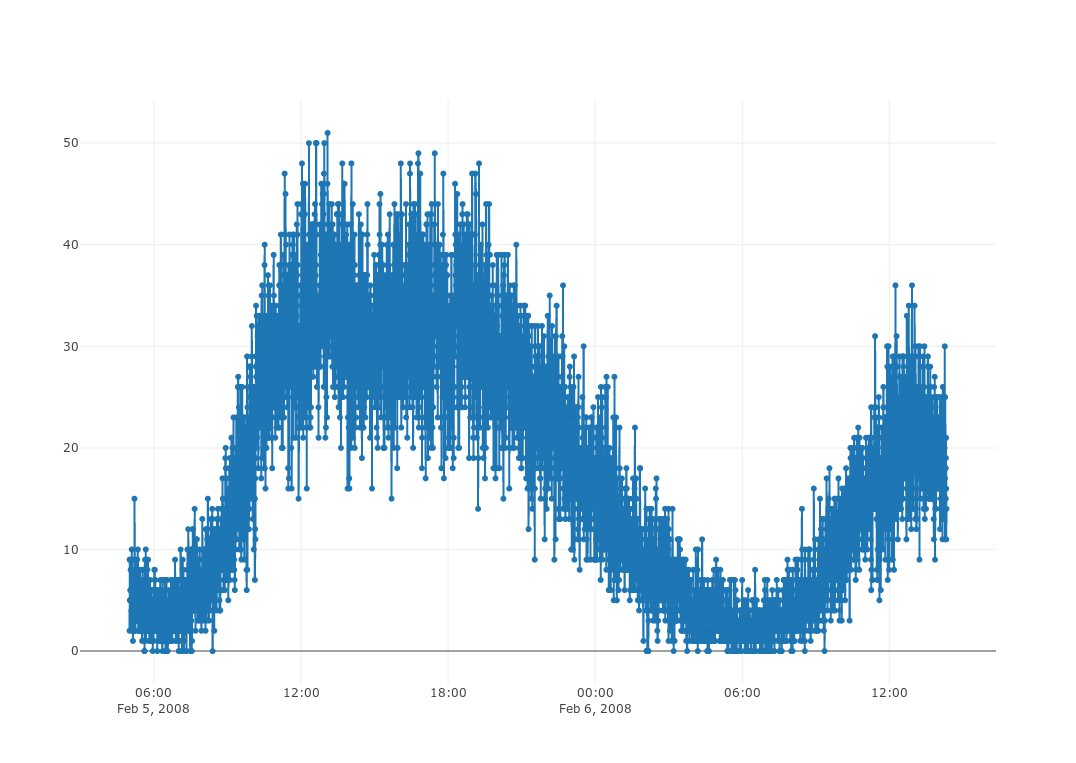
\includegraphics[width=1\textwidth]{img/20sec-feb5.png}
\end{center}
\end{frame}




\begin{frame}\frametitle{Experimental Setup}

We deployed a model checker (computation logic) and the current topology (static state) as a RESTful microservice. \\
Three alternative architectures:
\begin{itemize}
\item \textbf{Lambda Functions}: 3Gb RAM (vCPU quotas are assigned accordingly)
\item \textbf{Single Instance  of a Big VM}: Standard F64s\_v2 (64 vcpus, 128 GB memory)
\item \textbf{Autoscaling Group}: 5 to 20 t1.micro VMs (1Gb Ram, 1vCPU each)
\end{itemize}
Positions tracker (dynamic state) deployed as another standalone microservice

\end{frame}



\begin{frame}\frametitle{Execution Sample}


\begin{itemize}
\item \textbf{One hour window} of the Beijing dataset as workload (536 data points), the beginning of a daily peak 
\item \textbf{Time multipliers}: To simulate events that happen closer to each other.
    \begin{itemize}
    \item  5x / 10x / 20x / 40x / 60x time multipliers.
\end{itemize}

\item Run the experiment combining the different time multipliers with the three alternative deployments
% \item Defined a SLA of 30 seconds/call maximum
\end{itemize}

\begin{exampleblock}{Service Level Agreement }
Defined a SLA of 30 seconds/call maximum for responding to model checking requests
\end{exampleblock}
\end{frame}



\begin{frame}{Experimental Results}
    \begin{columns}[T]
        \begin{column}{0.57\textwidth}
            \vskip1.4cm
            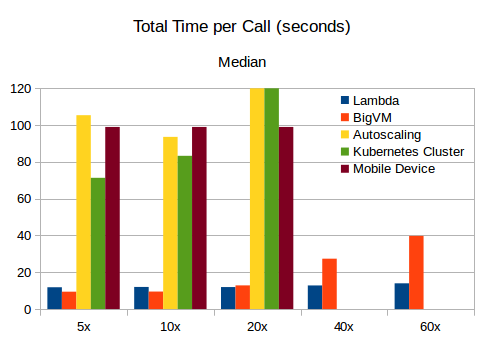
\includegraphics[width=\textwidth]{img/1.png}
        \end{column}
        \begin{column}{0.5\textwidth}
            \begin{itemize}
                \item The Autoscaling group had the \textbf{worst performance}. Requests timed out (504) with 20x time or more.
\item Lambda held an almost \textbf{constant performance} (~12s/call) for all workloads
\item The BigVM \textbf{(baseline)} performed better (9-12s) up to 20x, then started to decrease performance.
            \end{itemize}
        \end{column}
    \end{columns}
\end{frame}

\begin{frame}{Experimental Results}

\begin{figure}
   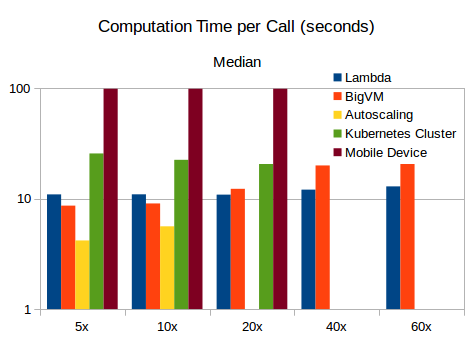
\includegraphics[width=0.49\textwidth]{img/2.png}
   \hfill
   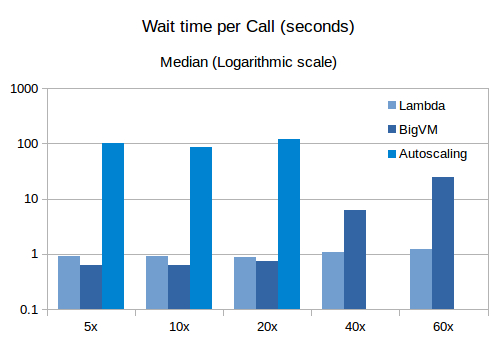
\includegraphics[width=0.49\textwidth]{img/3.png}
\end{figure}

\end{frame}


\begin{frame}{Experimental Results}

\begin{figure}
   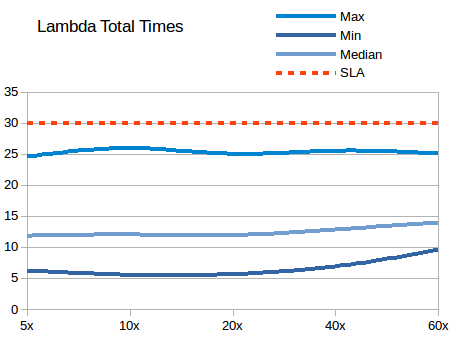
\includegraphics[width=0.49\textwidth]{img/4.png}
   \hfill
   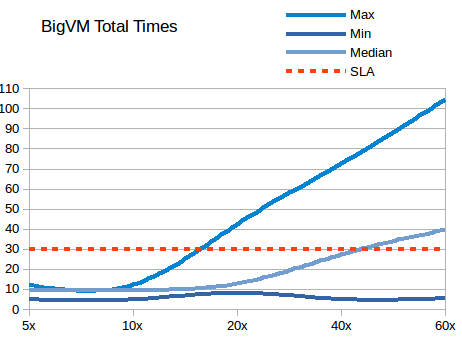
\includegraphics[width=0.49\textwidth]{img/5.png}
\end{figure}

\end{frame}





\begin{frame}\frametitle{Experimental Results: Discussion}


\begin{itemize}
\item Lambda functions kept a \textbf{constant performance} even under dense workloads, being more reactive and scalable.
\item The BigVM used as a baseline performed well for medium workloads, but not against peaks or more dense workloads \\ \textbf{(e.g. workloads unknown beforehand)}.

\item The autoscaling group did not seem suitable, but more experimentation is needed (fine-tuning parameters, scaling containers?).
\item Cost analysis to come (if the workload is more or less known, lambda could become more costly in comparison)
\end{itemize}
\end{frame}




\setbeamerfont{bibliography item}{size=\footnotesize}
\setbeamerfont{bibliography entry author}{size=\footnotesize}
\setbeamerfont{bibliography entry title}{size=\footnotesize}
\setbeamerfont{bibliography entry location}{size=\footnotesize}
\setbeamerfont{bibliography entry note}{size=\footnotesize}















\end{document}




















